\section{Results}
In this section we present our results from the experiments. The experiments follow the same order as they were presented in the previous section.


\subsection{Response time distribution}

\clearpage

\begin{figure}[h]
    \centering
    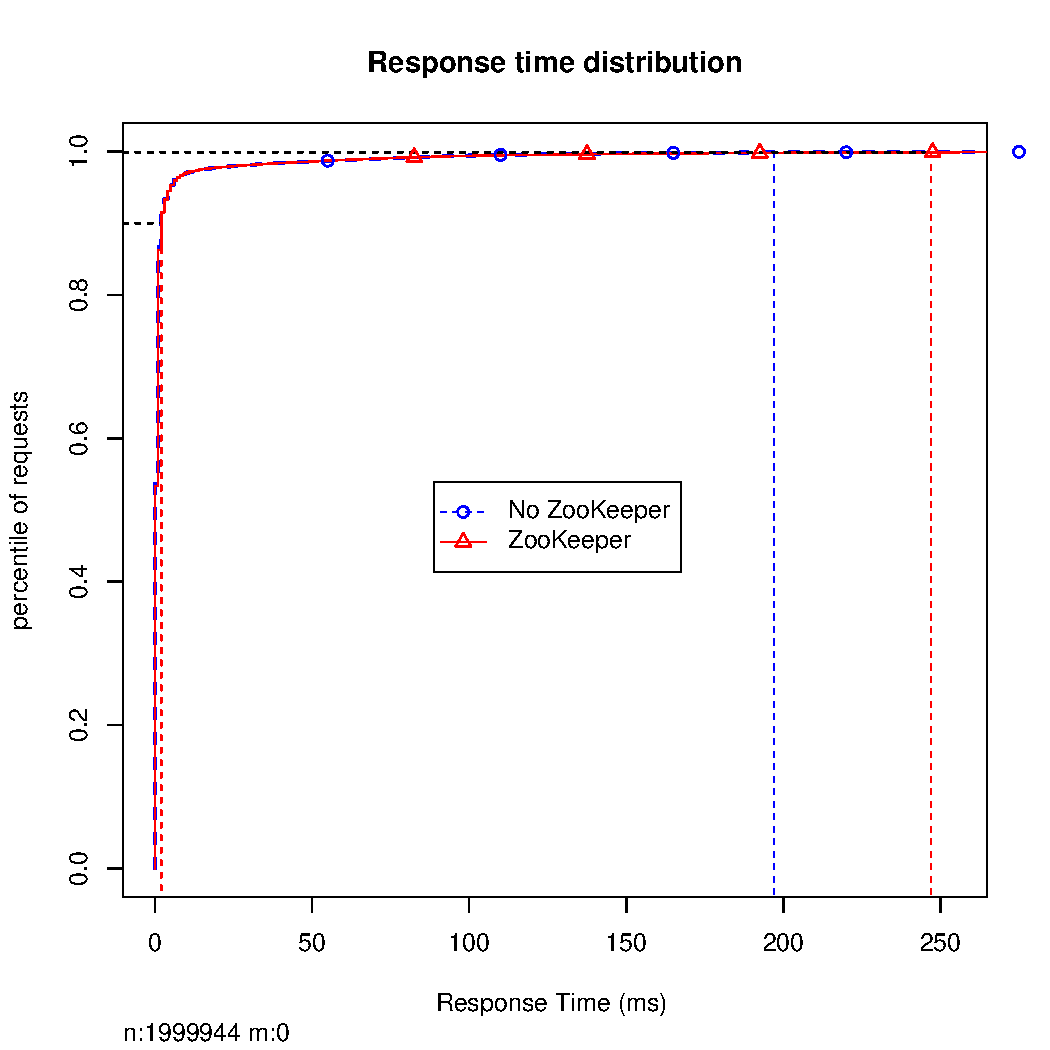
\includegraphics[width=1.0\textwidth]{results/distribution/distribution_macmini}
    \caption{Response time distribution Core 2 Duo Mac mini running both original code and our ZooKeeper implementation}
    \label{fig:dist_mini}
\end{figure}

From Figure \ref{fig:dist_mini} we see that both systems perform similarly on the Mac mini. The vertical lines mark the 0.9 and 0.999 percentile of requests. We see that 90\% of the requests are serviced within 2 ms while at the .999 percentile the response time is at 197 ms for our implementation and 247 ms for the original code.  

\clearpage

\begin{figure}[h]
    \centering
    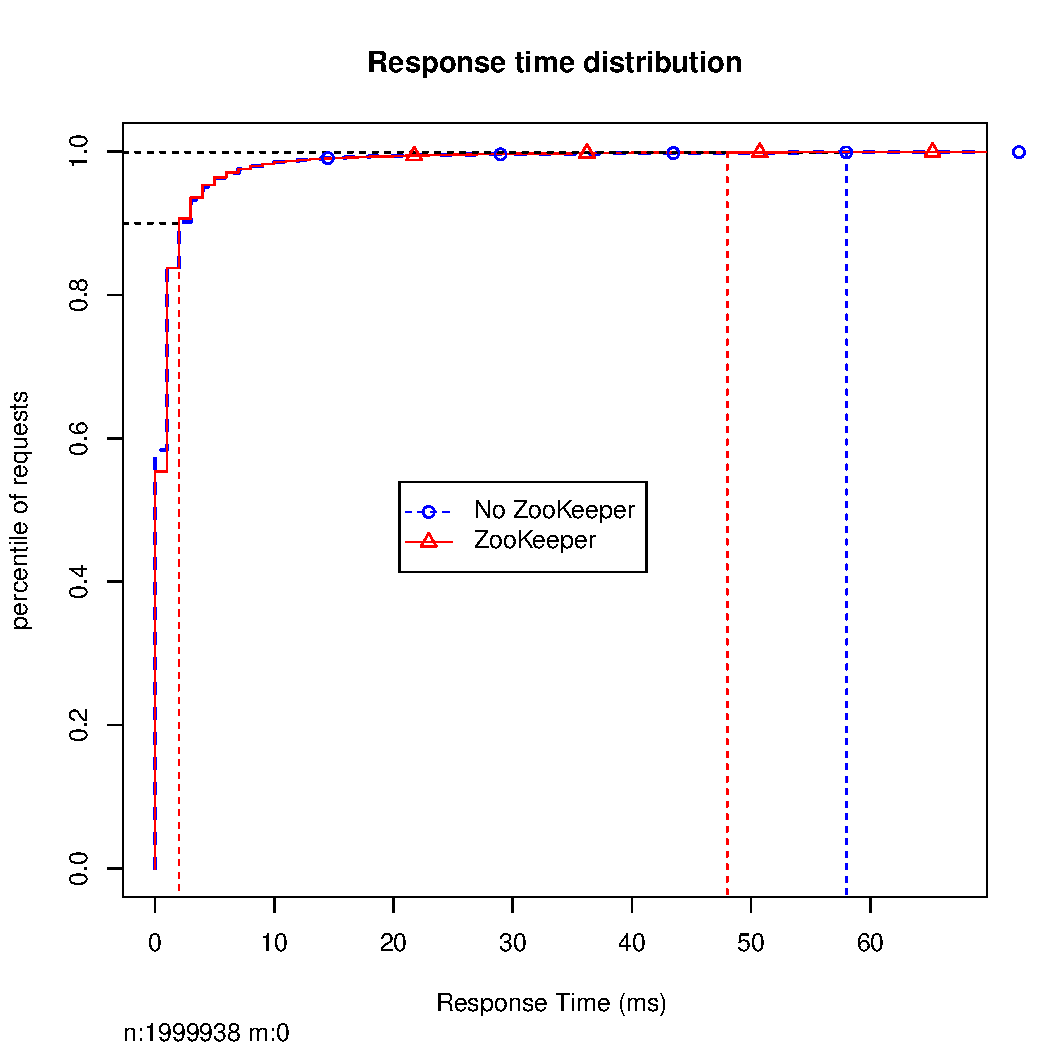
\includegraphics[width=1.0\textwidth]{results/distribution/distribution_knut}
    \caption{Response time distribution i5 MacBook running both original code and our ZooKeeper implementation}
    \label{fig:dist_knut}
\end{figure}

From Figure \ref{fig:dist_knut} we see that both systems still perform similarly on the i5 MacBook Pro. The vertical lines again mark the 0.9 and 0.999 percentile of requests. At the 0.90 percentile we see no improvement, however at the 0.999 percentile we see a massive improvement with 58 ms on our ZooKeeper implementation and 48 ms on the original code.  

\clearpage

\begin{figure}[h]
    \centering
    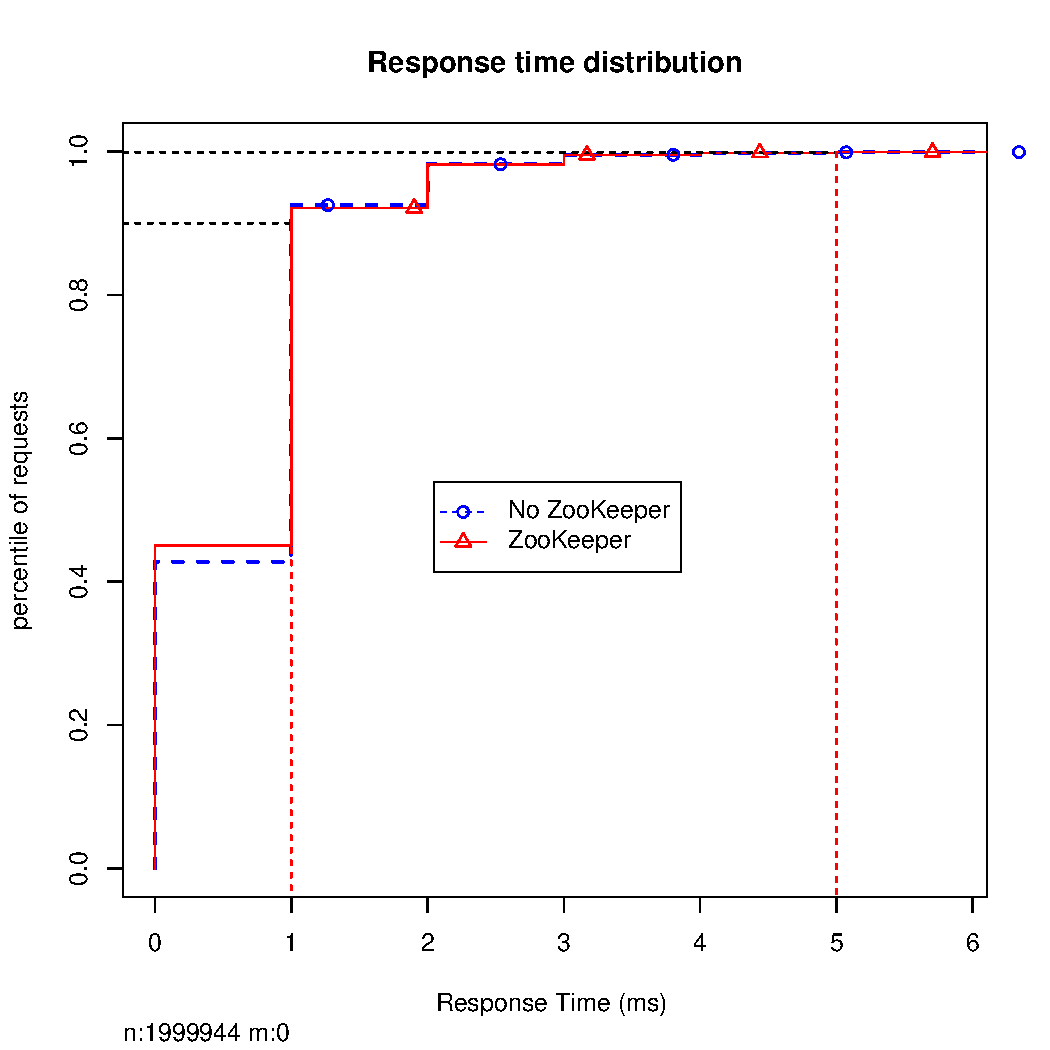
\includegraphics[width=1.0\textwidth]{results/distribution/distribution_eivind}
    \caption{Response time distribution i7 MacBook running both original code and our ZooKeeper implementation}
    \label{fig:dist_eivind}
\end{figure}

Finally in Figure\ref{fig:dist_eivind} we see the results on the i7 Macbook Pro. Again we see both implementations of Voldemort performing equally. At the 0.90 percentile the system responds in 1 ms in both cases and again we see a great increase in performance at the 0.999 percentile with 5 ms for both systems.

\subsection{Throughput}

\clearpage

\begin{figure}[h]
    \centering
    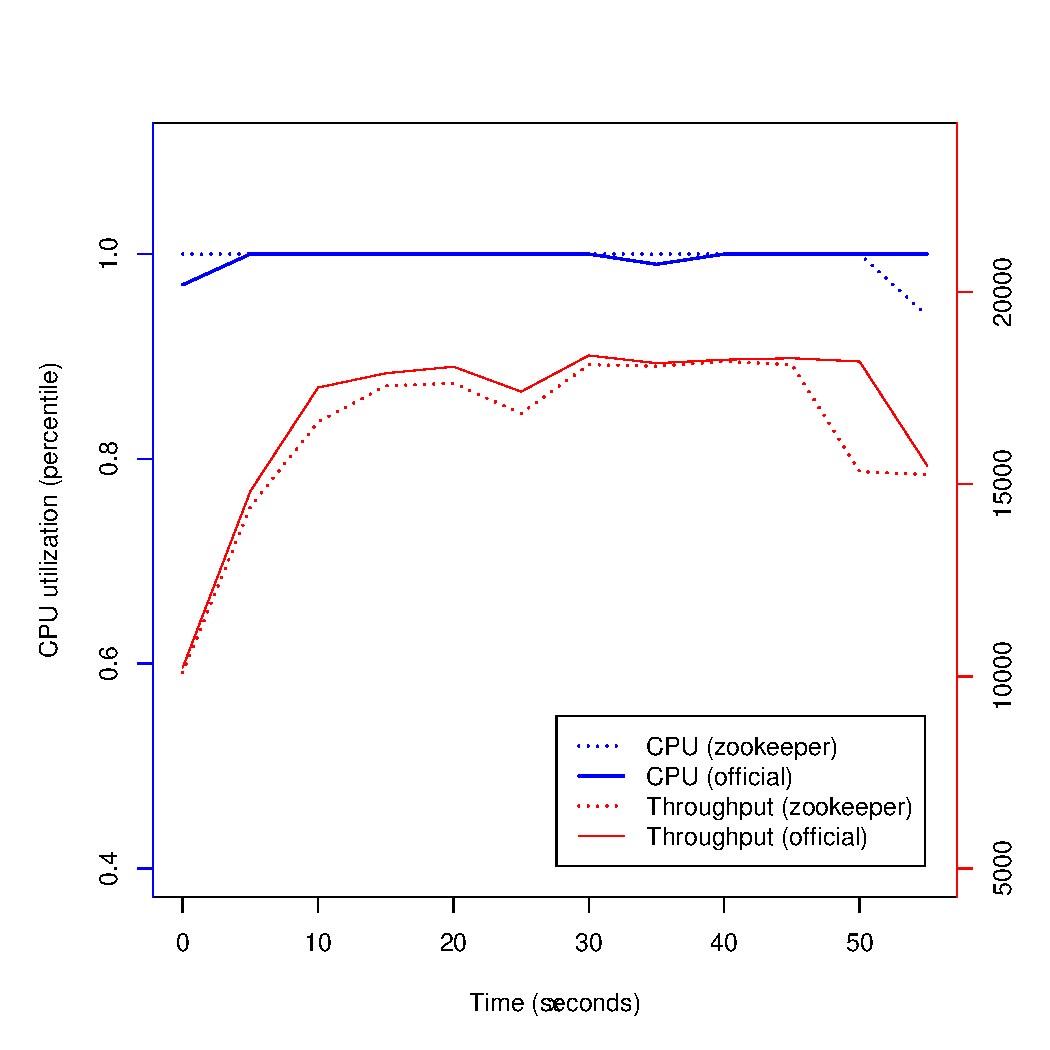
\includegraphics[width=1.0\textwidth]{results/throughput/singlenode/throughput_macmini}
    \caption{Throughput and CPU-load under stress test on Mac Mini}
    \label{fig:thug_mini}
\end{figure}

On Figure\ref{fig:thug_mini} we see that the Mac mini. The mini is clearly struggling to keep up with the workload running at close to 100\% utilization of the CPU. Maximum throughput seems to average around 17 000 requests per second.  

\clearpage

\begin{figure}[h]
    \centering
    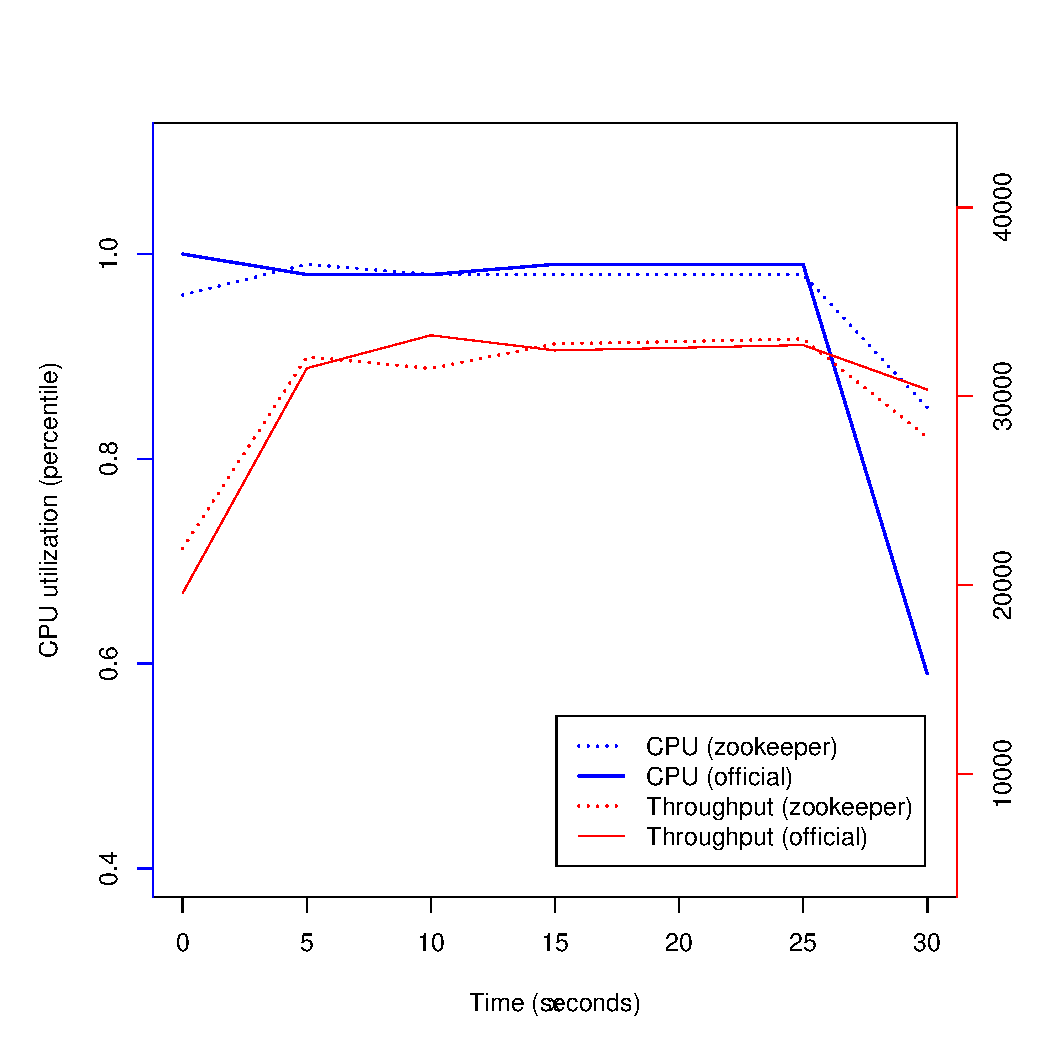
\includegraphics[width=1.0\textwidth]{results/throughput/singlenode/throughput_knut}
    \caption{Throughput and CPU-load under stress test on i5 MacBook Pro}
    \label{fig:thug_knut}
\end{figure}

\clearpage

\begin{figure}[h]
    \centering
    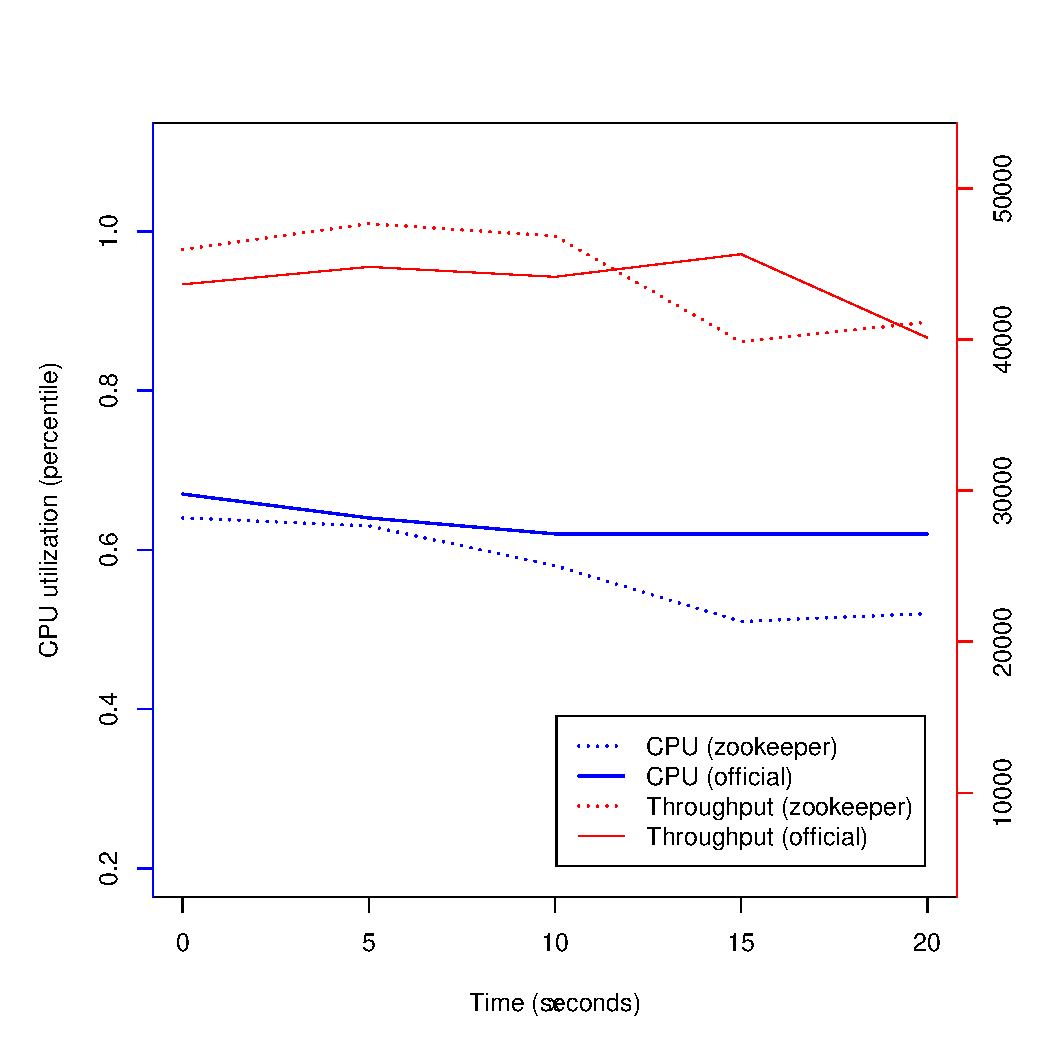
\includegraphics[width=1.0\textwidth]{results/throughput/singlenode/throughput_eivind}
    \caption{Throughput and CPU-load under stress test on i7 MacBook Pro}
    \label{fig:thug_eivind}
\end{figure}



% \begin{figure}[h]
%     \centering
%     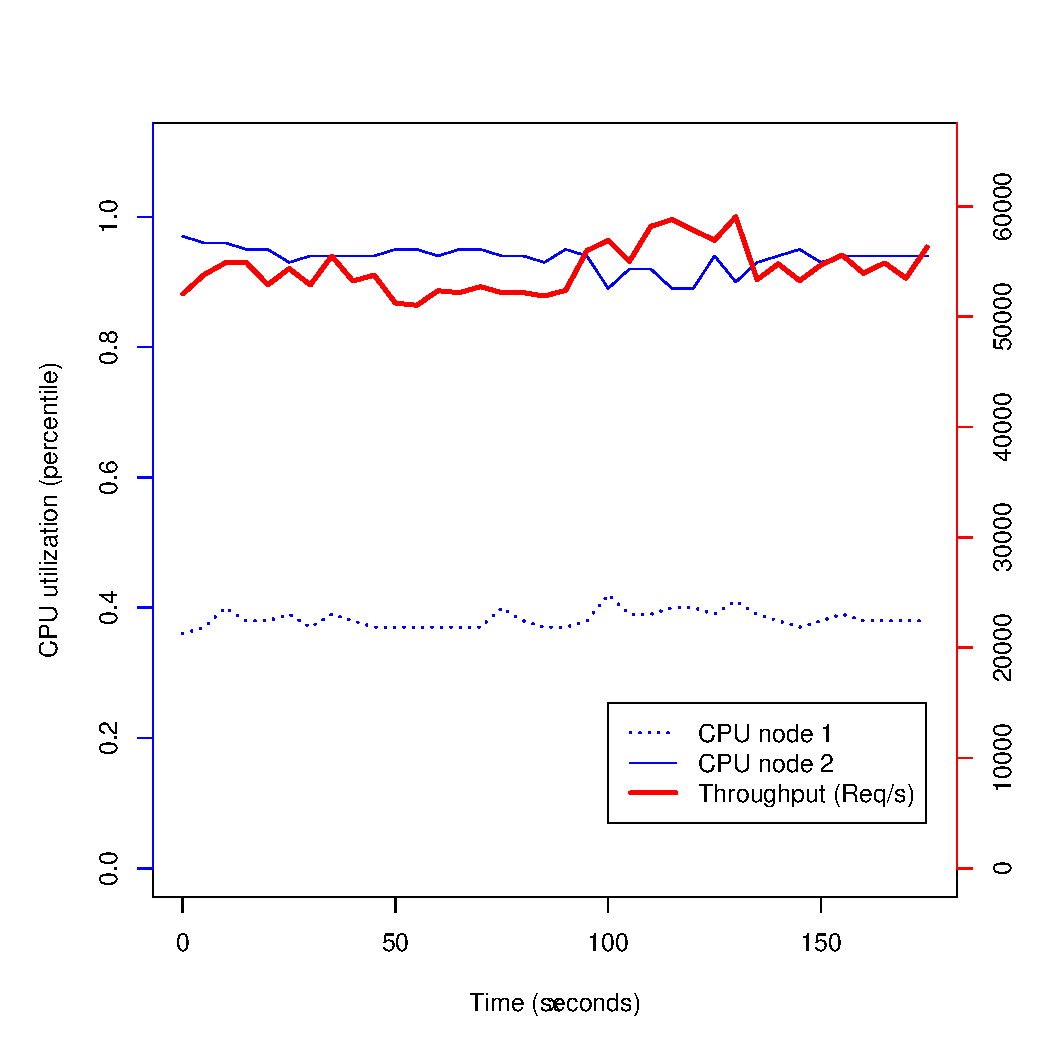
\includegraphics[width=1.2\textwidth]{results/baseline_originalsrc_v182}
%     \caption{Baseline for original source code. 2 heterogeneous Nodes, 8 partitions each.}
%     \label{fig:baseline}
% \end{figure}

% \begin{figure}[h]
%     \centering
%     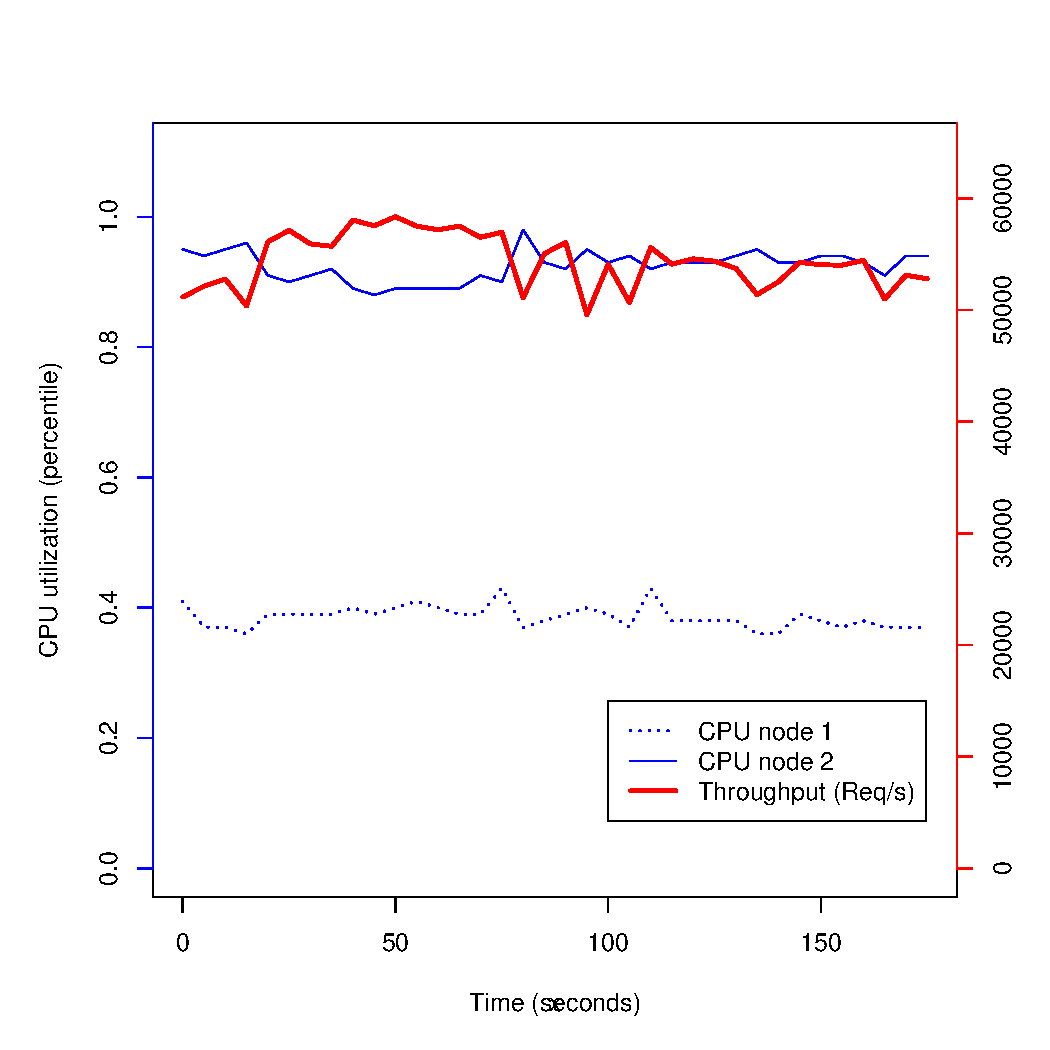
\includegraphics[width=1.2\textwidth]{results/baseline_plot}
%     \caption{Baseline for our modified source. 2 heterogeneous nodes, 8 partitions each.}
%     \label{fig:baseline}
% \end{figure}

% \begin{figure}[h]
%     \centering
%     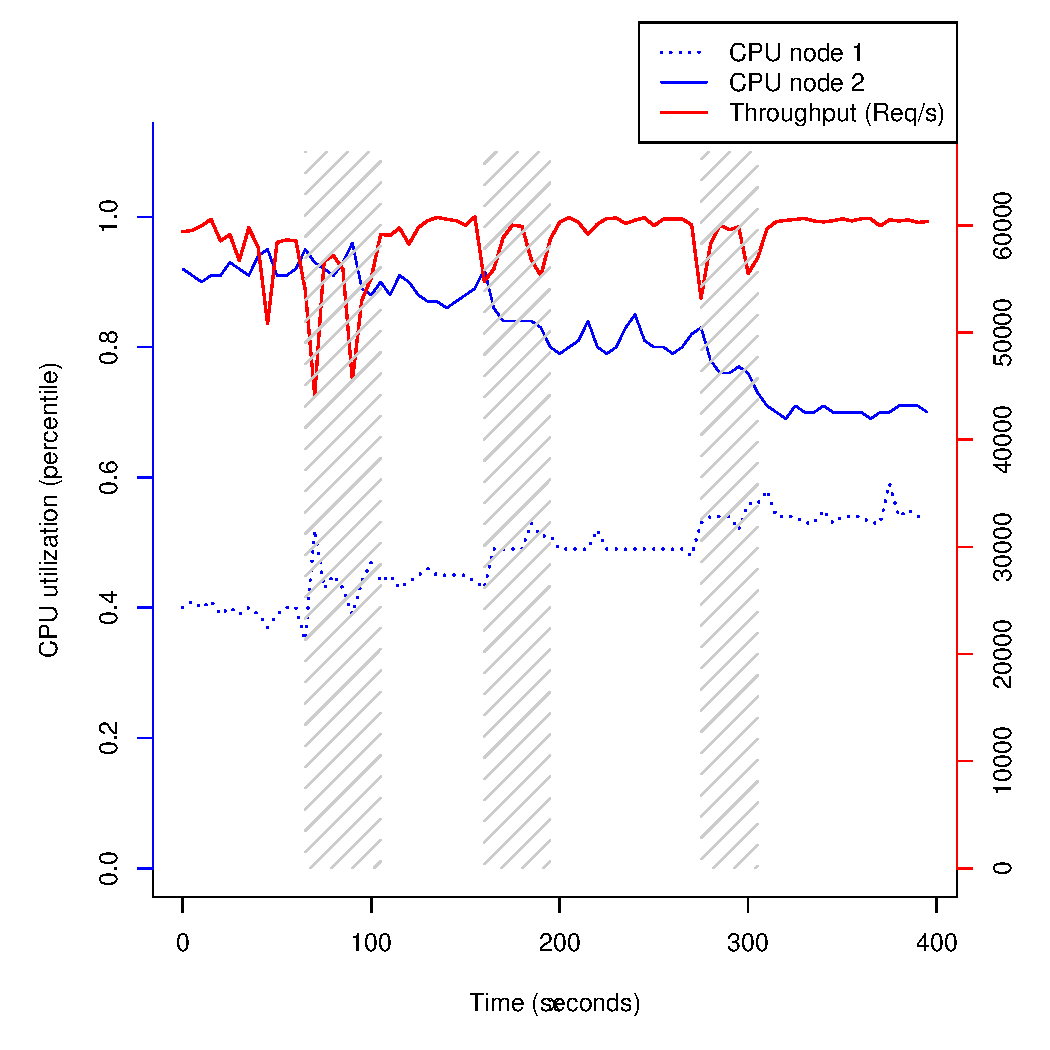
\includegraphics[width=1.2\textwidth]{results/rebalance_originalsrc}
%     \caption{Manual moving of 3 partitions from a struggling node (Node 2). Grey regions mark rebalance period, where data is prepared and transferred between nodes.}
%     \label{fig:adaptive}
% \end{figure}

% \begin{figure}[h]
%     \centering
%     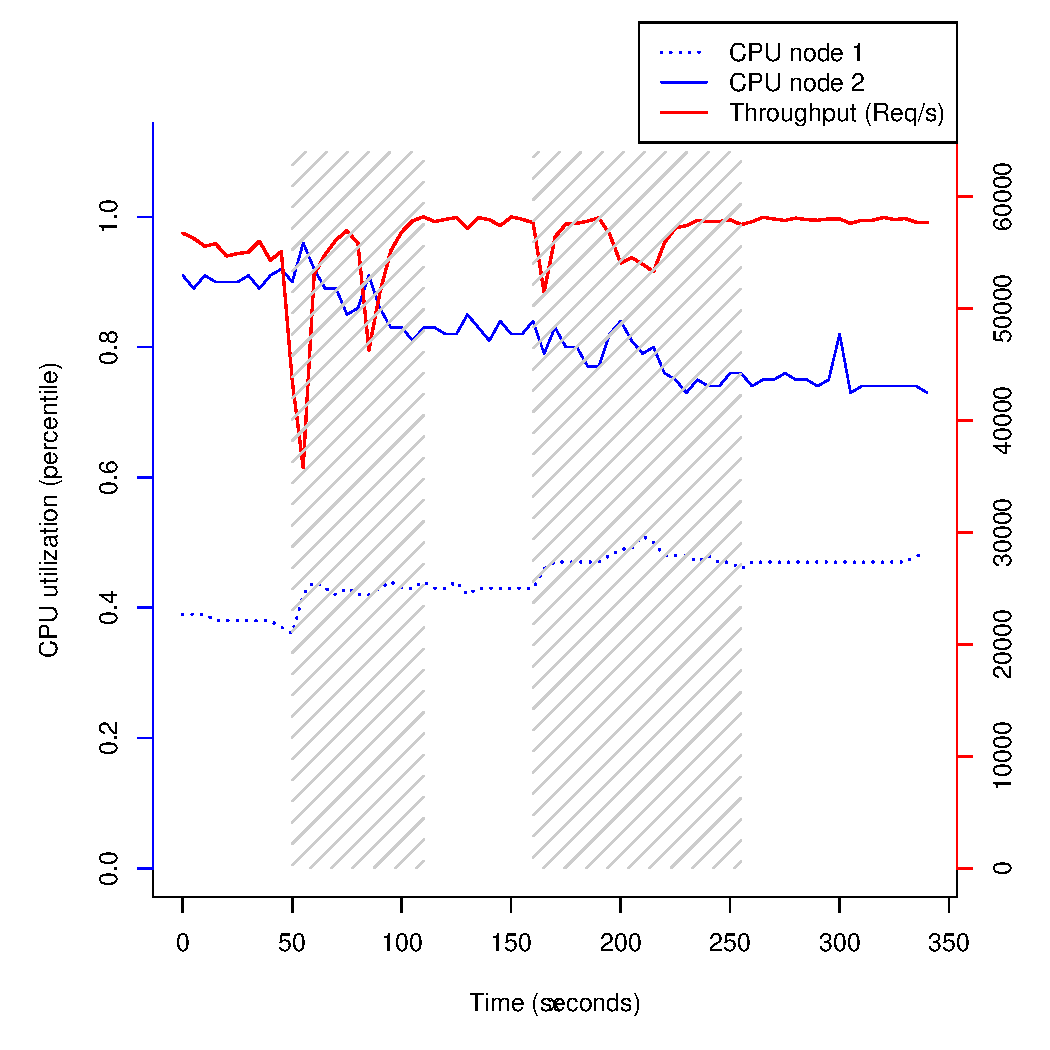
\includegraphics[width=1.2\textwidth]{results/adaptive_plot}
%     \caption{Automatic moving of 2 partitions from a struggling node (Node 2). Grey regions mark rebalance period, where data is prepared and transferred between nodes. CPU threshold set at \texttt{0.8}.}
%     \label{fig:adaptive}
% \end{figure}

